\documentclass[11pt,a4paper]{article}
\usepackage[margin=2.3cm]{geometry}
\usepackage{amsmath,amssymb,amsthm}
\usepackage{graphicx}
\usepackage{float}
\usepackage{caption}
\captionsetup[table]{position=top,skip=6pt}
\usepackage{enumitem}
\usepackage[hidelinks]{hyperref}
\emergencystretch=3em

\theoremstyle{definition}
\newtheorem{lemma}{Lemma}
\newcommand{\C}{\mathbb{C}}
\DeclareMathOperator*{\argmin}{arg\,min}
\DeclareMathOperator{\sgn}{sgn}

\title{Personal Meeting: Thermal-Noise Robustness of Sparse Refinement}
\date{October 19, 2026}
\author{}

\begin{document}
\maketitle

\section{Noise Model}

\subsection{Received Signal and SNR Definition}

The received echo is
\begin{equation}\label{eq:y}
  \mathbf Y = \mathbf S + \mathbf W,\qquad W_{mn} \overset{\text{i.i.d.}}{\sim} \mathcal{CN}(0,\sigma^2),
\end{equation}
where $\mathbf S$ is the noise-free echo and $\mathbf W$ is receiver thermal noise
(circularly symmetric complex Gaussian white noise). The SNR is defined on the noise-free
CSA image $\mathbf H_S = \mathrm{CSA}(\mathbf S)$ over the $800\times800$ scene $\Omega$:
\begin{equation}\label{eq:snr}
  \mathrm{SNR}_{\mathrm{dB}} = 10\log_{10}\frac{P_S}{\sigma^2},\qquad
  P_S = \frac{1}{|\Omega|}\sum_{(i,j)\in\Omega} |H_{S,ij}|^2 .
\end{equation}
Since the CSA is unitary, $\mathrm{CSA}(\mathbf W)$ is again i.i.d.\ $\mathcal{CN}(0,\sigma^2)$, so
adding the noise to the echo or to the focused image is equivalent.

\subsection{Relation to NESZ}

\begin{equation}\label{eq:nesz}
  \mathrm{SNR}_{\mathrm{dB}} \approx \overline{\sigma^0}_{\mathrm{dB}} - \mathrm{NESZ}_{\mathrm{dB}},
\end{equation}
where $\overline{\sigma^0}_{\mathrm{dB}}$ is the scene-averaged backscattering coefficient (averaged in
the linear-power domain, consistent radiometric calibration).

\subsection{Related Work}

Gao et al.~\cite{gao2024} model noisy TomoSAR observations as $\mathbf G = \mathbf A\boldsymbol\Gamma + \mathbf E$, with
i.i.d.\ zero-mean Gaussian noise $\mathbf E$ added to the focused data, and evaluate SNR from 0 to 20 dB
by Monte Carlo simulation. Our study instead adds the noise to the raw echo before CSA focusing.

\section{Experimental Setup}

\subsection{Dataset and Tuning Protocol}

All methods use the same protocol (Table~\ref{tab:protocol}).

\begin{table}[H]
\centering
\caption{Tuning and testing protocol.}\label{tab:protocol}
\begin{tabular}{|l|l|}
\hline
Item & Configuration \\
\hline
Dataset & HRSID (1,593 scenes) \\
\hline
Tuning set & 100 fixed scenes \\
\hline
Test set & 1,493 independent scenes \\
\hline
Primary objective & Maximize mAP@0.5 \\
\hline
Tie-breaking & F1-score if mAP difference $\le 0.002$ \\
\hline
Final tie-breaking & Prefer smaller parameters \\
\hline
Boundary handling & Expand the search range if the optimum lies on a boundary \\
\hline
\end{tabular}
\end{table}

\subsection{Evaluation Metrics}

Precision $=\mathrm{TP}/(\mathrm{TP}+\mathrm{FP})$ and Recall $=\mathrm{TP}/(\mathrm{TP}+\mathrm{FN})$ (Table~\ref{tab:confusion}).

\begin{table}[H]
\centering
\caption{Confusion matrix.}\label{tab:confusion}
\begin{tabular}{|l|c|c|}
\hline
 & Predicted Ship & Predicted Non-Ship \\
\hline
Actual Ship & TP & FN \\
\hline
Actual Non-Ship & FP & TN \\
\hline
\end{tabular}
\end{table}

\section{Results}

\subsection{Detection Performance vs SNR}

CSA shows high precision ($\approx 0.98$) but low recall (0.53 at $\infty$ to 0.14 at $-5$ dB): detected
ships are mostly correct, but weak ships are missed (Fig.~\ref{fig:metrics}). The three regularizations keep
recall above 0.81; $\ell_{1/2}+\mathrm{TV}$ is the highest at $-5$ dB (recall 0.883, mAP@0.5 0.943, Fig.~\ref{fig:reg}).

\begin{figure}[H]
\centering
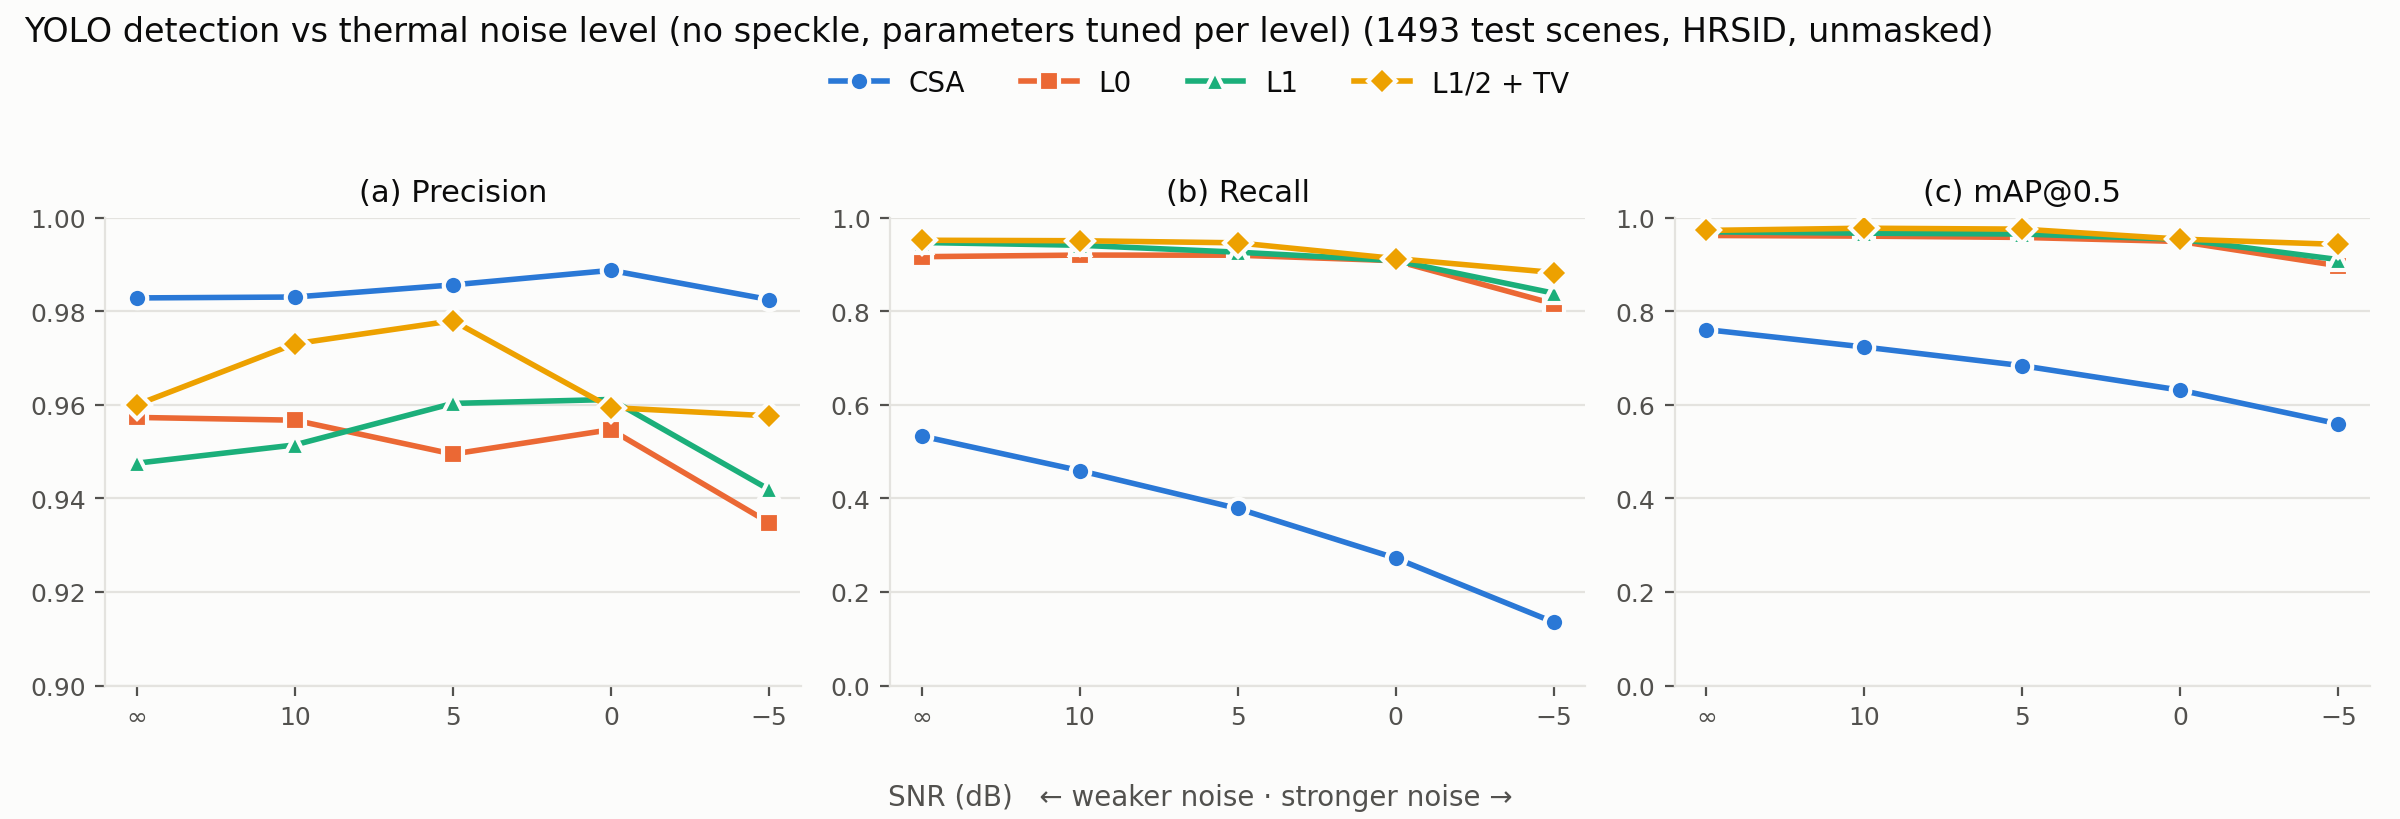
\includegraphics[width=\textwidth]{figures/metrics_vs_snr.png}
\caption{Precision, recall and mAP@0.5 vs SNR (parameters tuned per SNR level).}\label{fig:metrics}
\end{figure}

\begin{figure}[H]
\centering
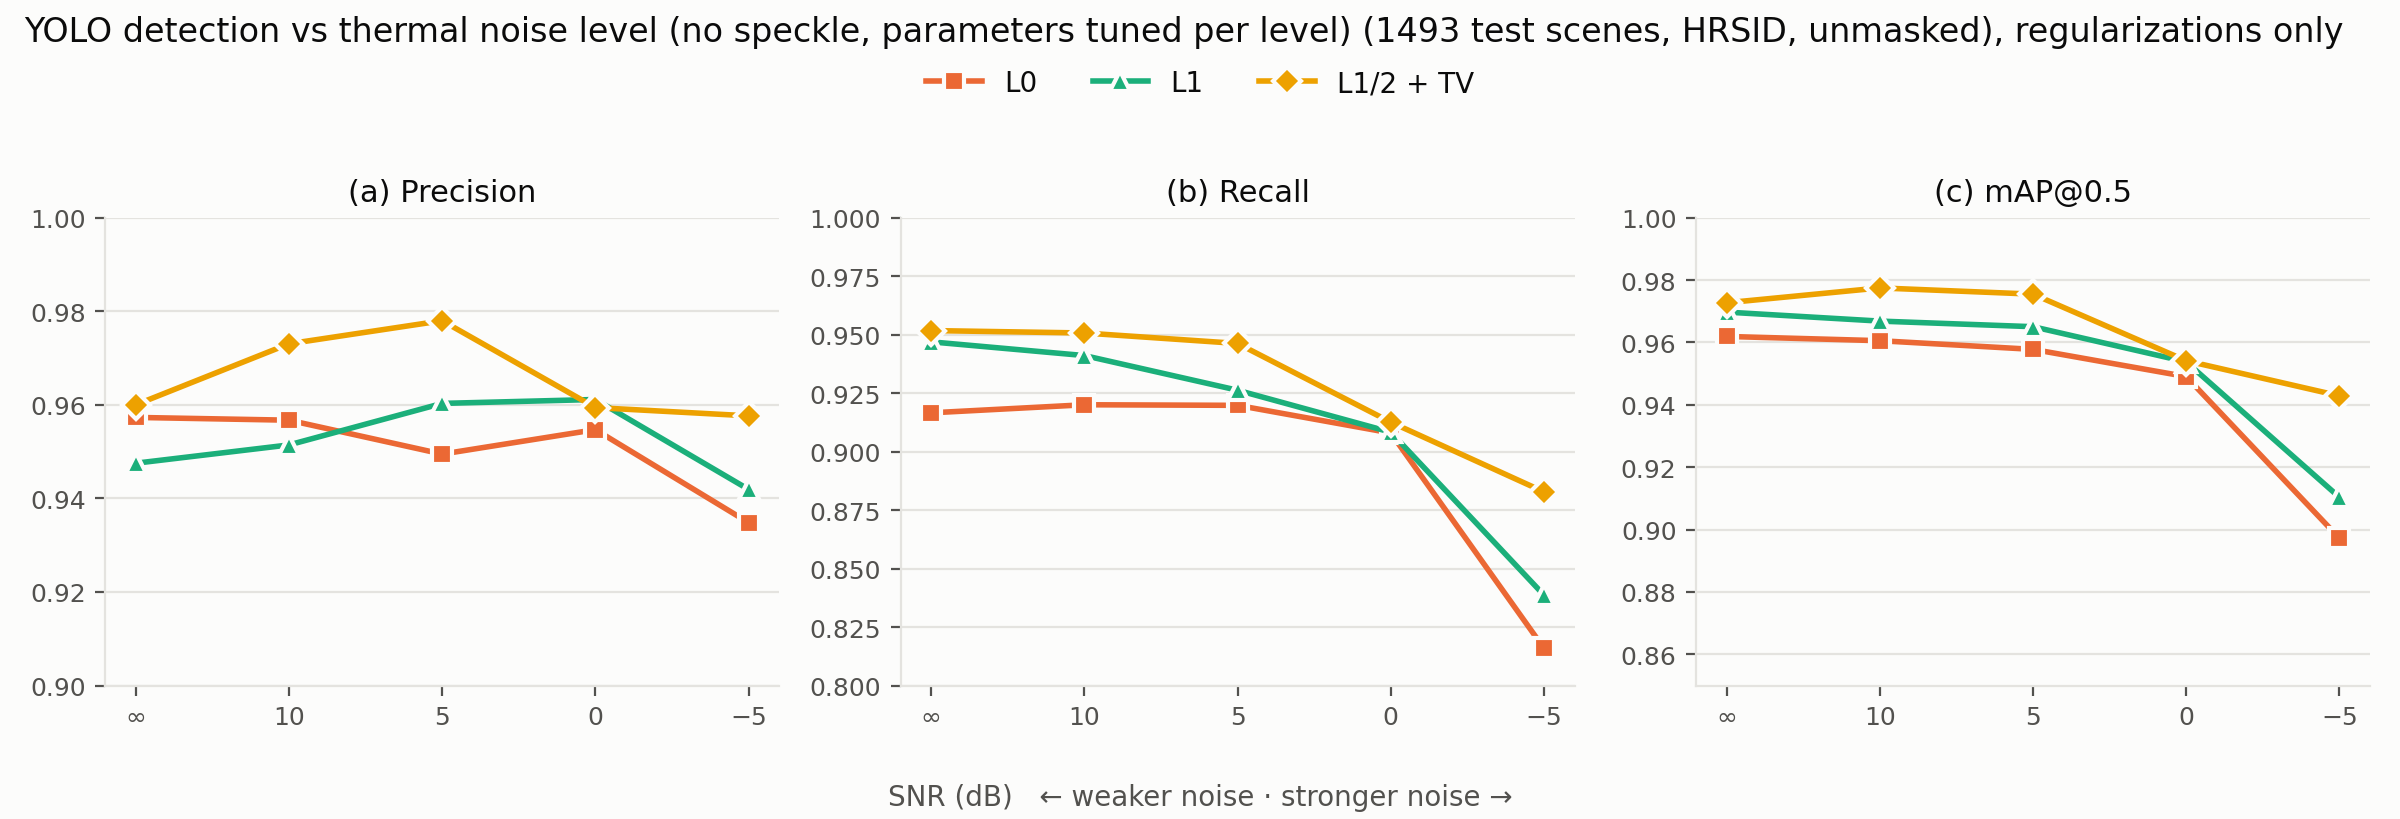
\includegraphics[width=\textwidth]{figures/metrics_vs_snr_regularization.png}
\caption{Same as Fig.~\ref{fig:metrics}, regularizations only.}\label{fig:reg}
\end{figure}

\subsection{Example}

\begin{figure}[H]
\centering
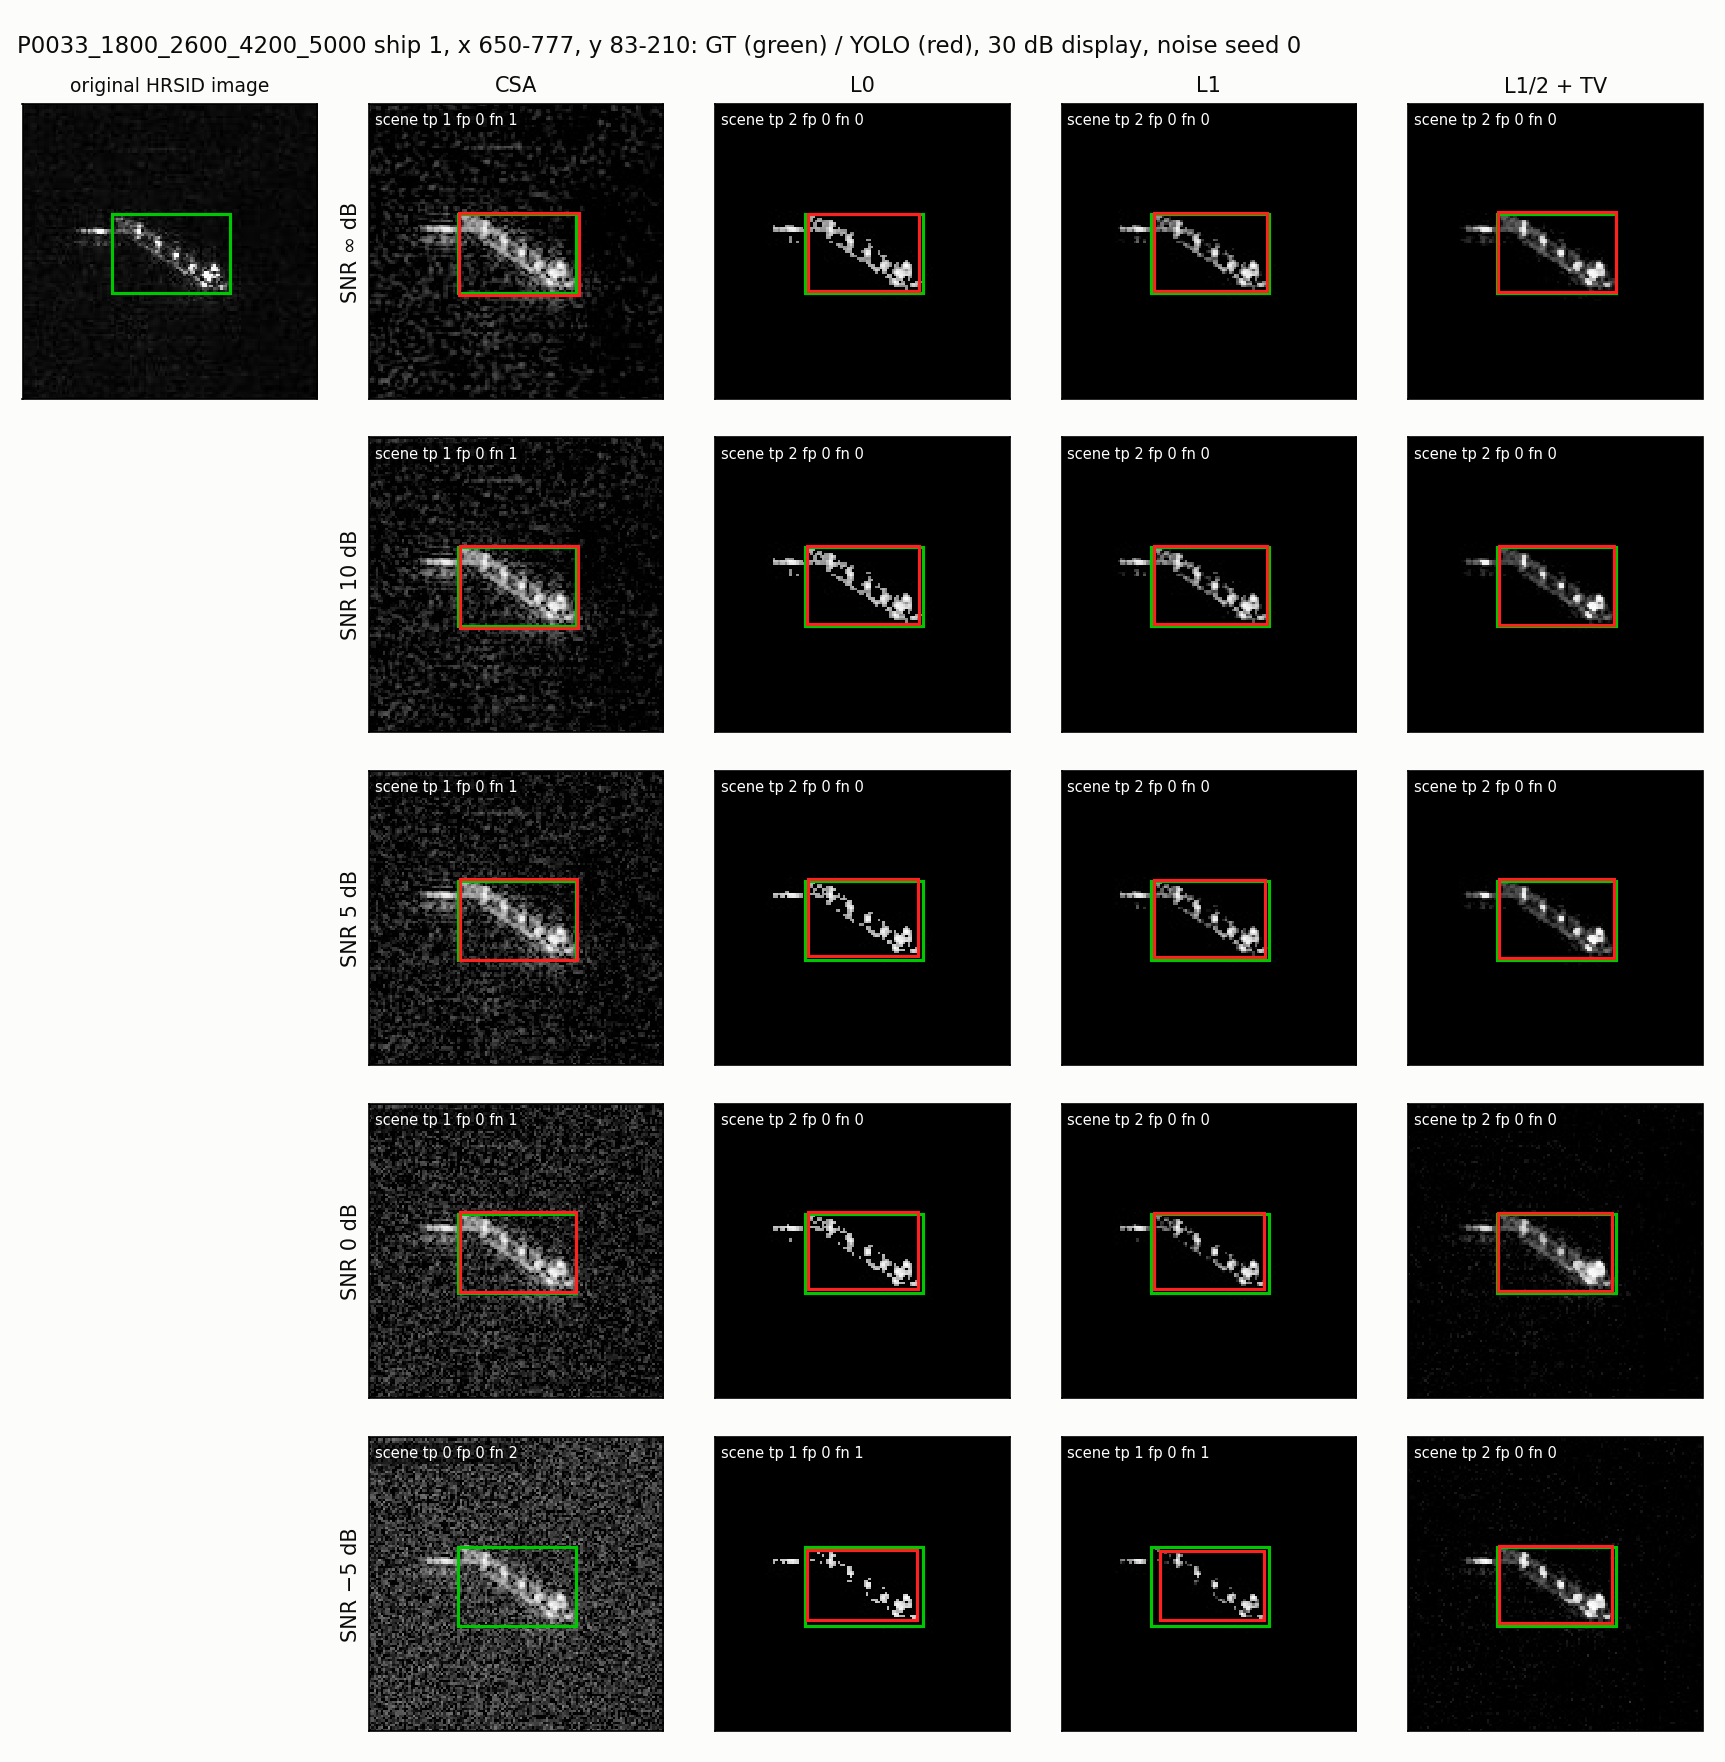
\includegraphics[width=0.8\textwidth]{figures/example_zoom_P0033_1800_2600_4200_5000_ship1.png}
\caption{Scene P0033\_1800\_2600\_4200\_5000, ship 1: GT (green) and YOLO (red) boxes.}\label{fig:example}
\end{figure}

\subsection{Selected Parameters}

\begin{table}[H]
\centering
\caption{Parameters selected per SNR level.}\label{tab:params}
\begin{tabular}{|l|c|c|c|c|c|}
\hline
SNR & $\ell_0$: $\alpha$ & $\ell_1$: $\alpha$ & $\ell_{1/2}+\mathrm{TV}$: $\alpha$ & $\xi$ & $\lambda_{TV}$ \\
\hline
$\infty$ & 0.20 & 0.13 & 0.13 & 2 & 0.03 \\
\hline
10 dB & 0.20 & 0.13 & 0.13 & 3 & 0.03 \\
\hline
5 dB & 0.25 & 0.16 & 0.13 & 3 & 0.03 \\
\hline
0 dB & 0.25 & 0.20 & 0.08 & 3 & 0.10 \\
\hline
$-5$ dB & 0.35 & 0.30 & 0.08 & 3 & 0.03 \\
\hline
\end{tabular}
\end{table}

\begin{itemize}
  \item $\ell_0/\ell_1$: higher noise levels require stronger thresholding (Appendix~\ref{app:thresholding}).
  \item $\ell_{1/2}+\mathrm{TV}$: noise is suppressed by regularization and smoothing while weaker ship
        responses are retained; moderate $\xi$ (2--3) gives stable convergence.
\end{itemize}

\subsection{Parameter Robustness}

Fixed: parameters tuned at $\infty$ and applied to all SNR levels. Adaptive: tuned per SNR level.

\begin{table}[H]
\centering
\caption{Test-set mAP@0.5, fixed vs adaptive parameters.}\label{tab:robust}
\begin{tabular}{|l|l|c|c|c|}
\hline
SNR & Method & Fixed & Adaptive & Gain \\
\hline
0 dB & $\ell_0$ & 0.916 & 0.949 & $+0.033$ \\
\hline
 & $\ell_1$ & 0.931 & 0.954 & $+0.023$ \\
\hline
 & $\ell_{1/2}+\mathrm{TV}$ & 0.954 & 0.954 & 0.000 \\
\hline
$-5$ dB & $\ell_0$ & 0.788 & 0.897 & $+0.109$ \\
\hline
 & $\ell_1$ & 0.810 & 0.910 & $+0.100$ \\
\hline
 & $\ell_{1/2}+\mathrm{TV}$ & 0.911 & 0.943 & $+0.032$ \\
\hline
\end{tabular}
\end{table}

$\ell_{1/2}+\mathrm{TV}$ shows the strongest parameter robustness.

\subsection{Convergence}

Average iterations of $\ell_{1/2}+\mathrm{TV}$ (tolerance $10^{-4}$, cap 300; all runs converged).

\begin{table}[H]
\centering
\caption{Average number of iterations of $\ell_{1/2}+\mathrm{TV}$.}\label{tab:iter}
\begin{tabular}{|l|l|c|}
\hline
SNR & Parameters & Average \\
\hline
$\infty$ & $\alpha = 0.13,\ \xi = 2,\ \lambda_{TV} = 0.03$ & 75 \\
\hline
10 dB & $\alpha = 0.13,\ \xi = 3,\ \lambda_{TV} = 0.03$ & 93 \\
\hline
5 dB & $\alpha = 0.13,\ \xi = 3,\ \lambda_{TV} = 0.03$ & 90 \\
\hline
0 dB & $\alpha = 0.08,\ \xi = 3,\ \lambda_{TV} = 0.1$ & 81 \\
\hline
$-5$ dB & $\alpha = 0.08,\ \xi = 3,\ \lambda_{TV} = 0.03$ & 56 \\
\hline
\end{tabular}
\end{table}

\begin{thebibliography}{1}
\bibitem{gao2024}
S. Gao, W. Wang, M. Wang, Z. Zhang, Z. Yang, X. Qiu, B. Zhang, and Y. Wu,
``A robust super-resolution gridless imaging framework for UAV-borne SAR tomography,''
\emph{IEEE Trans.\ Geosci.\ Remote Sens.}, vol.~62, Art.~no.~5210917, pp.~1--17, 2024.
\end{thebibliography}

\clearpage
\appendix
\setcounter{equation}{0}
\renewcommand{\theequation}{\thesection.\arabic{equation}}

\section{Derivation of Soft and Hard Thresholding}\label{app:thresholding}

This appendix derives the soft ($\ell_1$) and hard ($\ell_0$) thresholding operators used by the
$\ell_1$ and $\ell_0$ methods in the experiments above.

\subsection{Problem and Reduction to a Magnitude Problem}

Let $\mathbf z = (z_1,\dots,z_N)^{\mathsf T}\in\C^N$ be the observed complex image and
$\mathbf x\in\C^N$ the estimate. For $w\in\C$, $|w|$ is the modulus and
$\sgn(w) = w/|w|$ ($\sgn(0)=0$). In polar form,
$x_i = \rho_i e^{j\theta_i}$ and $z_i = m_i e^{j\varphi_i}$, with $\rho_i,m_i\ge0$.
For $\lambda>0$,
\begin{equation}\label{eq:problem}
  \hat{\mathbf x} = \argmin_{\mathbf x\in\C^N}
  \tfrac12\lVert \mathbf x - \mathbf z\rVert_2^2 + \lambda R(\mathbf x),
\end{equation}
where $\lVert\mathbf v\rVert_2^2 = \sum_i |v_i|^2$ and $R:\C^N\to[0,\infty)$ is a regularizer.

\begin{lemma}[Separability]\label{lem:sep}
Assume $R$ is separable over the entries, $R(\mathbf x) = \sum_{i=1}^N R_i(x_i)$ with
$R_i:\C\to[0,\infty)$. The data term is separable as well,
$\lVert\mathbf x-\mathbf z\rVert_2^2 = \sum_i|x_i-z_i|^2$, so the objective of~\eqref{eq:problem}
is $\sum_i J_i(x_i)$ with $J_i(x) = \tfrac12|x-z_i|^2 + \lambda R_i(x)$, and each
$\hat x_i = \argmin_{x\in\C} J_i(x)$ is found independently.
\end{lemma}

Drop the index $i$. With $x=\rho e^{j\theta}$ and $z = m e^{j\varphi}$,
\begin{equation}\label{eq:cos}
  |x - z|^2 = \rho^2 + m^2 - 2\rho m\cos(\theta-\varphi).
\end{equation}

\begin{lemma}[Phase]\label{lem:phase}
Assume further that each $R_i$ depends only on the modulus, $R_i(x) = r(|x|)$ for some
$r:[0,\infty)\to[0,\infty)$ with $r(0)=0$. Then for fixed $\rho>0$ the penalty does not depend
on $\theta$, and~\eqref{eq:cos} is smallest at $\theta=\varphi$, where $|x-z|^2 = (\rho-m)^2$.
\end{lemma}

Combining Lemmas~\ref{lem:sep} and~\ref{lem:phase}, the minimizer keeps the phase of $z$ and
thresholds its magnitude:
\begin{equation}\label{eq:mag}
  \hat x = \sgn(z)\,\hat\rho,\qquad
  \hat\rho = \argmin_{\rho\ge 0}\; g(\rho),\qquad
  g(\rho) = \tfrac12(\rho - m)^2 + \lambda r(\rho),\quad m = |z| .
\end{equation}

\subsection{\texorpdfstring{$\ell_1$}{L1}: Soft Thresholding}

$R(\mathbf x) = \lVert\mathbf x\rVert_1 = \sum_i |x_i|$ satisfies Lemmas~\ref{lem:sep} and~\ref{lem:phase} with $r(\rho) = \rho$.
Then $g(\rho) = \tfrac12(\rho-m)^2 + \lambda\rho$ is convex on $\rho\ge0$, with
$g'(\rho) = \rho - m + \lambda$.
If $m>\lambda$, then $g'=0$ at $\rho = m-\lambda>0$.
If $m\le\lambda$, then $g'>0$ for all $\rho>0$, so the minimizer is $\rho=0$.
Hence $\hat\rho = \max(m-\lambda,0)$:
\begin{equation}\label{eq:soft}
  \mathcal S_\lambda(z) = \sgn(z)\,\max(|z|-\lambda,\,0)
  = \begin{cases} \bigl(|z|-\lambda\bigr)\dfrac{z}{|z|}, & |z|>\lambda,\\[1ex] 0, & |z|\le\lambda.\end{cases}
\end{equation}
Retained entries are shrunk by $\lambda$ in magnitude.

\subsection{\texorpdfstring{$\ell_0$}{L0}: Hard Thresholding}

$R(\mathbf x) = \lVert\mathbf x\rVert_0 = \#\{i: x_i\neq 0\}$ counts the nonzero entries. Since
$x_i\neq0 \Leftrightarrow |x_i|>0$, it satisfies Lemmas~\ref{lem:sep} and~\ref{lem:phase} with $r(\rho) = \mathbf 1[\rho>0]$, and
$g(\rho) = \tfrac12(\rho-m)^2 + \lambda\,\mathbf 1[\rho>0]$. Compare the two cases:
$\rho=0$ gives $g(0) = \tfrac12 m^2$; for $\rho>0$ the penalty is constant, so the
best value is $\rho = m$, with $g(m) = \lambda$. $\rho=m$ is better iff
$\lambda<\tfrac12 m^2$, i.e.\ $m>\sqrt{2\lambda}$:
\begin{equation}\label{eq:hard}
  \mathcal H_{\sqrt{2\lambda}}(z) = \begin{cases} z, & |z|>\sqrt{2\lambda},\\ 0, & |z|\le\sqrt{2\lambda}.\end{cases}
\end{equation}
At $|z|=\sqrt{2\lambda}$, both $0$ and $z$ are minimizers; \eqref{eq:hard} picks $0$.
Retained entries are unchanged.

\end{document}
